\documentclass[hyperref={pdfpagemode=FullScreen}]{beamer}
\usepackage{multicol}
\usepackage{ragged2e}
\usepackage{graphicx}
\usepackage{hyperref}
\usepackage{color}
\usepackage{colortbl}
\usetheme{Frankfurt}
\title{University of Lodz}
\author{Rashad Mahmudov}
\date{9 April 2020}

\begin{document}
\begin{frame}
\titlepage
\end{frame}

\begin{frame}{About}
\begin{block}{History}
  The University of Lodz is one of the leading institutions of higher education in Poland. 
  It was established in 1945 as a successor of educational institutions active in Lodz in earlier times. 
  The 12 faculties of the University provide programmes in 76 fields of study and 160 specializations.
\end{block}
\end{frame}

\begin{frame}{About}
\begin{block}{Students}
About 10,000 students complete their programmes at the University of Lodz every year. Our students, together with those studying in Lodz within Erasmus exchange, come from about 80 different countries.
\end{block}
\end{frame}

\begin{frame}{About}
\begin{block}{Languages}
The interest in studying at the University of Lodz is determined by high quality of instruction and modern programmes of study offered in Polish, English and French, and adapted to the changing demands of the labour market. 
\end{block}
\end{frame}

\begin{frame}{Facts \& Figures}
\centering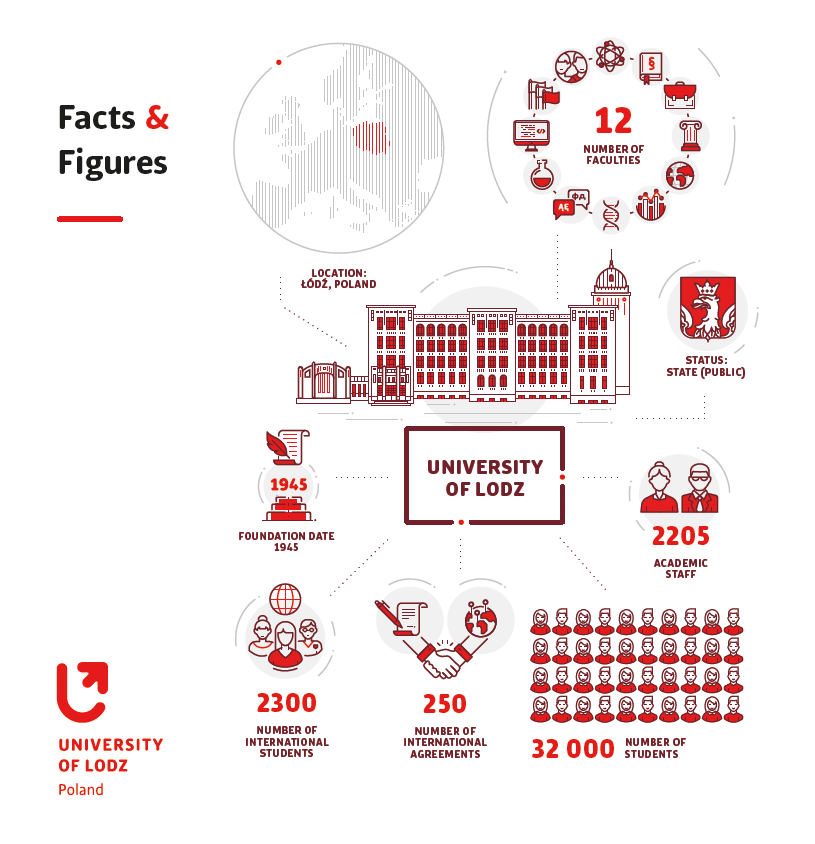
\includegraphics[scale=0.35]{img/pic1.png}\qquad
\end{frame}


\begin{frame}{Faculties}

\setlength{\columnsep}{0.5cm}
\begin{multicols}{2}
\newcommand{\mycommand}{\footnotesize\color{blue}\hspace{-1.5cm}}
\hspace{-4.1em}{
\includegraphics[scale=.27]{img/pic2.png}}

\vspace{5cm}{
\mycommand\href{http://www.biol.uni.lodz.pl/en/}{Faculty of Biology and Environmental Protection}}\\
 \mycommand\href{http://www.chemia.uni.lodz.pl/scientific_profile.html}{Faculty of Chemistry}\\
\mycommand\href{http://www.eksoc.uni.lodz.pl/en/}{Faculty of Economics and Sociology}\\
 \mycommand\href{http://www.wnow.uni.lodz.pl/}{Faculty of Educational Sciences}\\
 \mycommand\href{http://www.wnow.uni.lodz.pl/}{Faculty of Educational Sciences}\\ \mycommand\href{http://www.geo.uni.lodz.pl/}{Faculty of Geographical Sciences}\\
\mycommand\href{http://www.wsmip.uni.lodz.pl/wydzial?locale=en}{Faculty of International and Political Studies}\\
 \mycommand\href{https://www.wpia.uni.lodz.pl/en/research/research-centers}{Faculty of Law and Administration}\\ \mycommand\href{http://zarzadzanie.uni.lodz.pl/tabid/1562/Default.aspx}{Faculty of Management}\\ \mycommand\href{http://en.math.uni.lodz.pl/en/faculty-zone/}{Faculty of Mathematics and Computer Science}\\ \mycommand\href{http://filolog.uni.lodz.pl/}{Faculty of Philology}\\
\mycommand\href{http://wydzfilhist.uni.lodz.pl/}{Faculty of Philosophy and History}\\
\mycommand\href{http://faculty20of20physics20and20applied20informatics}{Faculty of Physics and Applied Informatics}


\end{multicols}
\end{frame}


\begin{frame}{Cooperation}
\begin{block}{International Cooperation}
The University of Lodz is involved in various international cooperation activities, including research and educational projects, student and faculty exchange within Erasmus+ and bilateral agreements, technology transfer, summer schools, as well as other numerous activities.
\end{block}
\begin{block}{International Cooperation Strategy}
 The range of existing cooperation includes mutual research projects, dual diplomas, and exchange of academic staff and students. In its strategy, the University of Lodz focuses on developing strong partnerships that foster long lasting and deep relationships worldwide.
\end{block}
\end{frame}


\begin{frame}{Poland}
\begin{columns}

\begin{column}{.5\textwidth}
\justifying The Republic of Poland is a country in Central Europe, bordered by Germany to the west, Czech Republic and Slovakia to the south, Ukraine and Belarus to the east, as well as Russia (Kaliningrad Oblast) and Lithuania to the northeast.).
\end{column}

\begin{column}{.5\textwidth}
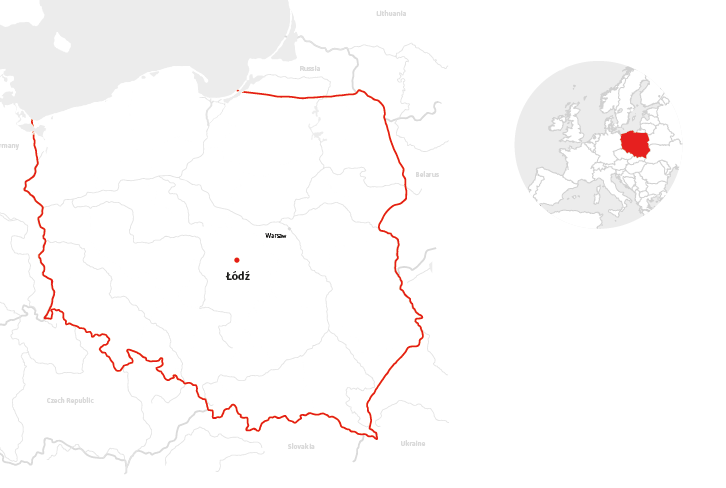
\includegraphics[scale=.30]{img/pic3.png}
\end{column}

\end{columns}
\end{frame}


\begin{frame}{Lodz}
\begin{columns}

\begin{column}{.5\textwidth}
\begin{itemize}
    \item\footnotesize\textbf{Capital of the region}
    \item\footnotesize{City rights in \textbf{1423}}
    \item\footnotesize{Poland’s \textbf{3rd largest city by population}}
    \item\footnotesize{Poland’s \textbf{4th largest city by area}}
    \item\footnotesize{\textbf{Before 1989} – textile and cinematography industry center}
    \item\footnotesize{\textbf{Today} – cultural, industrial and academic centre}
    \item\footnotesize\textbf{Safe city}
\end{itemize}
\end{column}

\begin{column}{.5\textwidth}
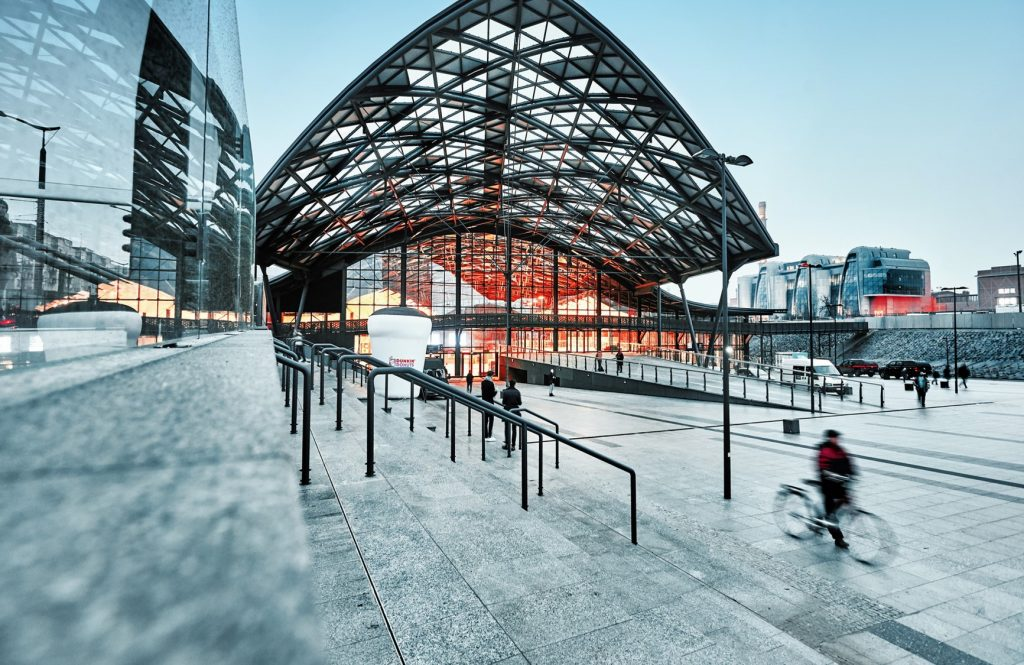
\includegraphics[scale=.21]{img/pic4.jpg}
\end{column}
\end{columns}
\end{frame}


\begin{frame}{End}
\begin{center}
\Huge\textbf{Thank you for attention!}
\end{center}
\end{frame}

\end{document}

